\section{Introduction}

Bias benchmarks for large language models routinely allow a model to decline
to answer (by selecting an \textsc{unknown} option, saying ``cannot be
determined,'' or otherwise abstaining) and then report a score computed on
what remains. This is standard on BBQ's ambiguous-context items
\citep{parrish2022bbq} and on WinoGender-style coreference probes
\citep{rudinger2018gender}. It is also a specific threat to validity: if
abstention is not independent of the disposition being measured, the reported
score confounds what the model prefers with how willing it is to say so, and
no amount of additional data closes the gap. \citet{manski1989anatomy} gave
the general form of this problem for missing outcomes decades before it
became relevant here.

The concern is easy to state and easy to dismiss as theoretical. Our first
contribution is to show it is neither. BBQ's ambiguous bias score is defined
so that it is \emph{multiplied} by the complement of the abstention rate.
Since on ambiguous items the gold answer is the \textsc{unknown} option,
that complement is exactly the rate at which the model commits to an answer.
An intervention that only teaches a model to abstain more therefore drives
the reported score toward zero while telling us strictly less about the
model. Applying this decomposition to every method--model pair in the main
results table of a recent debiasing paper, we find a median 80.4\% of
reported improvement is this mechanical effect, and that the evaluation's
identified set widened in 31 of 32 cases: the reported success and the loss
of identification are the same event (Figure~\ref{fig:teaser}). We then establish the phenomenon
independently of any published harness, first-party on six checkpoints
across all eleven BBQ categories (\S\ref{sec:firstparty}). Abstention turns
out to be a property of the checkpoint and disposition a property of the
social category, so comparing checkpoints, which is what a leaderboard does,
ranks them substantially by abstention.

% GENERATED by make_paper_assets.py -- do not edit by hand.
\begin{figure}[t]
\centering
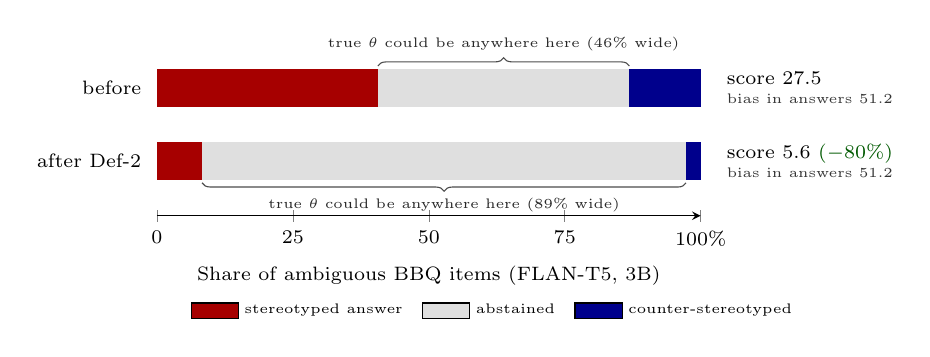
\begin{tikzpicture}
\begin{axis}[
  width=0.70\columnwidth, height=3.9cm, xmin=0, xmax=100, ymin=0.25, ymax=2.75,
  ytick={1,2}, yticklabels={after Def-2,before},
  xtick={0,25,50,75,100}, xticklabels={0,25,50,75,100\%},
  tick label style={font=\scriptsize}, label style={font=\scriptsize},
  xlabel={Share of ambiguous BBQ items (FLAN-T5, 3B)},
  axis lines=left, y axis line style={draw=none}, ytick style={draw=none},
  clip=false,
  legend columns=3, legend style={at={(0.62,-0.42)}, anchor=north, draw=none, font=\tiny,
    /tikz/every even column/.append style={column sep=5pt}},
]
\addlegendimage{area legend, draw=none, fill=red!65!black}\addlegendentry{stereotyped answer}
\addlegendimage{area legend, draw=none, fill=gray!25}\addlegendentry{abstained}
\addlegendimage{area legend, draw=none, fill=blue!55!black}\addlegendentry{counter-stereotyped}
\fill[red!65!black] (axis cs:0,1.74) rectangle (axis cs:40.63,2.26);
\fill[gray!25] (axis cs:40.63,1.74) rectangle (axis cs:86.89,2.26);
\fill[blue!55!black] (axis cs:86.89,1.74) rectangle (axis cs:100,2.26);
\draw[decorate, decoration={brace, amplitude=3pt}, gray!60!black] (axis cs:40.63,2.3) -- (axis cs:86.89,2.3) node[midway, above=2pt, font=\tiny, text=gray!30!black] {true $\theta$ could be anywhere here (46\% wide)};
\node[anchor=west, font=\scriptsize, align=left] at (axis cs:103,2) {score 27.5\\[-1pt]\textcolor{gray!40!black}{\tiny bias in answers 51.2}};
\fill[red!65!black] (axis cs:0,0.74) rectangle (axis cs:8.31,1.26);
\fill[gray!25] (axis cs:8.31,0.74) rectangle (axis cs:97.31,1.26);
\fill[blue!55!black] (axis cs:97.31,0.74) rectangle (axis cs:100,1.26);
\draw[decorate, decoration={brace, amplitude=3pt}, gray!60!black] (axis cs:97.31,0.7) -- (axis cs:8.31,0.7) node[midway, below=2pt, font=\tiny, text=gray!30!black] {true $\theta$ could be anywhere here (89\% wide)};
\node[anchor=west, font=\scriptsize, align=left] at (axis cs:103,1) {score 5.6 \textcolor{green!35!black}{($-80$\%)}\\[-1pt]\textcolor{gray!40!black}{\tiny bias in answers 51.2}};
\end{axis}
\end{tikzpicture}
\caption{Abstention masquerading as debiasing. A published intervention cuts
BBQ's ambiguous bias score by 80\% on FLAN-T5, yet bias among the answers
the model still gives is unchanged (51.21 to 51.18). The model
simply abstains more (46\% to 89\%).
Because the grey span is exactly the identified interval for the model's
disposition, the ``improvement'' is the benchmark losing sight of the model.}
\label{fig:teaser}
\end{figure}


If reported scores are compromised this way, the obvious response is to
re-elicit under a forced-choice policy, or against some instrument that
removes the model's ability to decline, and then check whether the
conditions agree. Our second contribution asks whether \emph{that} check is
itself sound, and finds that the natural implementation is not. We pose
agreement as a linear-programming compatibility certificate over an
arbitrary number of elicitation conditions (Figure~\ref{fig:method} maps both
analyses). Evaluated on plug-in proportions, it rejects a null with no
cross-condition structure 21.3\% of the time at 16 draws, and calibrated
against a null resampled from our own panel, more draws do not fix this: the
rate plateaus at 21--23\% out to 4{,}096 draws. An exact-binomial version has
a false-positive rate of at most 0.1\% at every draw count tested.

We run both versions on six instruction\hy{}tuned checkpoints from four
families, on all 480 eligible WinoGender items, using a
refusal\hy{}direction ablation \citep{arditi2024refusal} as a
refusal\hy{}ablated comparator. A per-model null explains 83--94\% of each
checkpoint's naive rejections. The corrected certificate isolates 29
violations: 25 implicate the comparator itself, including on a checkpoint
that never once abstains, so there is no refusal to remove, 3 are
consistent with genuine response\hy{}policy effects, and 1 is a
forced-condition outlier.

Our contributions are:
\begin{enumerate}[nosep]
\item An exact decomposition of BBQ ambiguous scores into coverage and
  disposition, applied to 32 published method--model pairs and replicated
  first-party on six checkpoints across eleven categories, showing that
  abstention lives in the checkpoint and disposition in the category, that
  abstainers still lean toward the stereotype, and that this survives
  rewording and extends to twelve checkpoints (2024--2026) and six languages
  (\S\ref{sec:decomposition}, \S\ref{sec:firstparty}, \S\ref{sec:multilingual}).
\item A compatibility certificate for $Z$ elicitation conditions posed as a
  linear program, with a necessary-dependence bound $\gamma^*$
  (\S\ref{sec:certificate}).
\item A calibration showing persistent false positives for the plug-in
  certificate under the tested null and sampling budgets, an exact-binomial
  correction, and a per-model null for assessing aggregate incompatibility
  counts (\S\ref{sec:calibration}).
\item Application to six checkpoints, including a taxonomy that distinguishes
  instrument failure from response-policy effects, and evidence that
  abstention leans toward unnamed referents in every checkpoint that abstains
  (\S\ref{sec:models}).
\end{enumerate}

All three tools are benchmark-agnostic. The identity holds for any score of
the form coverage times committed-answer bias, which covers BBQ and every
benchmark that adopts its ambiguous-context metric, and the certificate and
its calibration take any panel of elicitation conditions by answer categories,
whatever produced it. We demonstrate them on BBQ and WinoGender, the standard
selective-answer bias benchmarks with public items. Our critique targets a
metric definition and what can be concluded from it, not the interventions'
authors, who report accuracy and bias score exactly as the benchmark
specifies.

\begin{figure*}[t]
\centering
\begin{adjustbox}{max width=\textwidth}
\begin{tikzpicture}[
  x=1cm, y=1cm,
  box/.style={draw=black!45, rounded corners=2pt, fill=white, font=\scriptsize,
              align=center, inner sep=2.5pt},
  arr/.style={-{Stealth[length=1.5mm]}, line width=0.6pt, black!65},
  lab/.style={font=\scriptsize\bfseries, anchor=west},
]
% ---------------- top row: BBQ ----------------
\node[lab] at (-0.6,1.95) {BBQ};
\node[box, minimum width=1.9cm, minimum height=1.5cm] (q) at (0.35,0)
  {\textbf{Item}\\[1pt]ambiguous context,\\question, options};
\node[box, fill=gray!12, minimum width=1.2cm, minimum height=1.5cm] (llm) at (3.0,0) {LLM};
\node[box, fill=red!8, draw=red!50!black, minimum width=3.3cm] (ps) at (6.1,0.9)
  {stereotype answer\quad$p_s$};
\node[box, fill=blue!8, draw=blue!50!black, minimum width=3.3cm] (pc) at (6.1,0)
  {counter-stereotype\quad$p_c$};
\node[box, fill=gray!15, minimum width=3.3cm] (pu) at (6.1,-0.9)
  {unknown / abstain\quad$p_u$};
\node[box, minimum width=3.0cm, minimum height=1.9cm] (met) at (10.0,0)
  {coverage $c=p_s+p_c$\\[3pt]
   bias $b=\dfrac{p_s-p_c}{p_s+p_c}$\\[3pt]
   \fbox{$s_{\mathrm{AMB}}=c\times b$}};
\draw[arr] (q) -- (llm);
\draw[arr] (llm.east) -- ++(0.3,0) |- (ps.west);
\draw[arr] (llm.east) -- (pc.west);
\draw[arr] (llm.east) -- ++(0.3,0) |- (pu.west);
\draw[arr] (ps.east) -- ++(0.25,0) |- ([yshift=0.45cm]met.west);
\draw[arr] (pc.east) -- (met.west);
\draw[arr] (pu.east) -- ++(0.25,0) |- ([yshift=-0.45cm]met.west);
% identified interval, drawn schematically
\begin{scope}[shift={(12.95,-0.8)}]
  \fill[blue!14] (0,0.8) -- (2.2,1.75) -- (2.2,-0.15) -- cycle;
  \draw[blue!60!black, line width=0.8pt] (0,0.8) -- (2.2,0.62);
  \draw[black!55, dashed, line width=0.4pt] (0,0.8) -- (2.2,0.8);
  \draw[-{Stealth[length=1.2mm]}, black!70] (0,-0.15) -- (2.4,-0.15);
  \draw[-{Stealth[length=1.2mm]}, black!70] (0,-0.15) -- (0,1.9);
  \node[font=\tiny, anchor=north] at (0,-0.2) {0};
  \node[font=\tiny, anchor=north] at (2.2,-0.2) {1};
  \node[font=\tiny, anchor=north] at (1.1,-0.42) {abstention $p$};
  \node[font=\tiny, rotate=90, anchor=south] at (-0.12,0.85) {preference};
  \node[font=\scriptsize, align=center] at (1.1,2.35) {identified interval\\widens with $p$};
\end{scope}
\draw[arr] (met.east) -- (12.75,0);

% ---------------- bottom row: WinoGender ----------------
\node[lab] at (-0.6,-2.65) {WinoGender};
\node[box, minimum width=1.9cm, minimum height=1.5cm] (w) at (0.35,-4.6)
  {\textbf{Item}\\[1pt]sentence with a\\pronoun, two\\candidate referents};
\node[box, fill=orange!10, draw=orange!60!black, minimum width=3.2cm] (d) at (3.9,-3.7)
  {\textsc{direct} (may abstain)};
\node[box, fill=blue!8, draw=blue!50!black, minimum width=3.2cm] (f) at (3.9,-4.6)
  {\textsc{forced} (must choose)};
\node[box, fill=green!8, draw=green!40!black, minimum width=3.2cm] (r) at (3.9,-5.5)
  {\textsc{refusal-ablated}\\[-1pt]\tiny forced, refusal direction removed};
\node[font=\tiny, anchor=north] at (3.9,-6.05) {16 draws per condition};
\node[box, fill=gray!12, minimum width=1.0cm, minimum height=2.3cm] (par) at (6.55,-4.6)
  {shared\\parser};
\draw[arr] (w.east) -- ++(0.25,0) |- (d.west);
\draw[arr] (w.east) -- (f.west);
\draw[arr] (w.east) -- ++(0.25,0) |- (r.west);
\draw[arr] (d.east) -- ++(0.2,0) |- ([yshift=0.5cm]par.west);
\draw[arr] (f.east) -- (par.west);
\draw[arr] (r.east) -- ++(0.2,0) |- ([yshift=-0.5cm]par.west);
% condition x answer panel
\begin{scope}[shift={(9.05,-5.6)}]
  \foreach \i/\c in {0/green,1/blue,2/orange}{
    \foreach \j/\s in {0/60,1/22,2/10}{
      \fill[\c!\s] (\j*0.62,\i*0.62) rectangle +(0.6,0.6);}}
  \node[font=\tiny, anchor=east] at (-0.05,0.31) {refusal-abl.};
  \node[font=\tiny, anchor=east] at (-0.05,0.93) {forced};
  \node[font=\tiny, anchor=east] at (-0.05,1.55) {direct};
  \node[font=\tiny, rotate=40, anchor=south west] at (0.1,1.88) {occupation};
  \node[font=\tiny, rotate=40, anchor=south west] at (0.72,1.88) {participant};
  \node[font=\tiny, rotate=40, anchor=south west] at (1.34,1.88) {residual};
  \node[font=\scriptsize, align=center] at (0.93,-0.4) {condition $\times$ answer\\counts};
\end{scope}
\draw[arr] (par.east) -- (8.2,-4.6);
\node[box, minimum width=2.7cm, minimum height=1.7cm] (lp) at (12.85,-4.6)
  {exact-binomial\\lower bounds $\mathrm{lo}_z(k)$\\[3pt]
   LP test:\\$\sum_k \max_z \mathrm{lo}_z(k)\le 1$};
\draw[arr] (11.0,-4.6) -- (lp.west);
\node[box, fill=green!8, draw=green!40!black, minimum width=2.5cm] (ok) at (15.95,-3.85)
  {\textbf{compatible}\\[-1pt]\tiny shared answer law\\[-2pt]\tiny not rejected};
\node[box, fill=red!8, draw=red!50!black, minimum width=2.5cm] (bad) at (15.95,-5.35)
  {\textbf{incompatible}\\[-1pt]\tiny inspect the dissenting\\[-2pt]\tiny condition};
\draw[arr] (lp.east) -- ++(0.25,0) |- (ok.west);
\draw[arr] (lp.east) -- ++(0.25,0) |- (bad.west);
\end{tikzpicture}
\end{adjustbox}
\caption{\textbf{Overview of the two analyses.} \emph{Top (BBQ).} Repeated
completions on an ambiguous item give stereotype, counter-stereotype, and
abstain probabilities. The score factors as $s_{\mathrm{AMB}}=c\times b$
(coverage $c=p_s+p_c$, committed-answer bias $b=(p_s-p_c)/(p_s+p_c)$), and the
identified interval widens with the abstention rate $p$
(\S\ref{sec:decomposition}). \emph{Bottom (WinoGender).} The item is elicited
under \textsc{direct}, \textsc{forced}, and \textsc{refusal-ablated} conditions,
16 draws each. A shared parser builds a condition$\times$answer panel,
exact-binomial lower bounds feed a linear-program compatibility test
($\sum_k \max_z \mathrm{lo}_z(k)\le 1$), and the panel is compatible with one
answer law or certified incompatible, prompting inspection of the dissenting
condition (\S\ref{sec:certificate}--\S\ref{sec:models}).}
\label{fig:method}
\end{figure*}

